\documentclass[12pt,a4paper,openany]{book}
\usepackage{lmodern}
\usepackage[svgnames]{xcolor} % Required to specify font color
\input{../LaTexTemplate/templates/couleurs.tex}

\usepackage{makeidx}
\usepackage[utf8]{inputenc} 
\usepackage{marvosym}
\usepackage[T1]{fontenc}
\usepackage[francais]{babel}
\usepackage[top=1.7cm, bottom=1.7cm, left=1.7cm, right=1.7cm]{geometry}
\usepackage{verbatim}
\usepackage[urlbordercolor={1 1 1}, linkbordercolor={1 1 1}, linkcolor=vert1, urlcolor=bleu, colorlinks=true]{hyperref}
\usepackage{tikz} %Vectoriel
\usepackage{listings}
\usepackage{fancyhdr}
\usepackage{multido}
\usepackage{amssymb}
\usepackage{float}
\usepackage[francais]{minitoc}
\usepackage[final]{pdfpages} 
\usepackage{graphicx} % Required for box manipulation
\usepackage{makeidx}

\newcommand{\titre}{Plan d'Assurance Qualité Logicielle}
\newcommand{\subtitle}{Équipe FACT : Florent Berbie, Antoine de Roquemaurel, Cédric Rohaut, Andriamihary Manantsoa Razanajatovo
M1 Informatique (Semestre 8) | UE Projet
Université Toulouse III Paul Sabatier}
\newcommand{\auteur}{Équipe FACT : Florent Berbie, Antoine de Roquemaurel, Cédric Rohaut, Andriamihary Manantsoa Razanajatovo}
\newcommand{\semestre}{8}
\newcommand{\annee}{2015}


\newcommand{\pole}{}
\newcommand{\sigle}{FACT}
\makeindex
\usepackage[totoc]{idxlayout}


\input{../LaTexTemplate/templates/listings.tex}
\input{../LaTexTemplate/templates/classroomsTemplates/l2/cours.tex}
\input{../LaTexTemplate/templates/remarquesExempleAttention.tex}
\input{../LaTexTemplate/templates/polices.tex}
\input{../LaTexTemplate/templates/affichageChapitre.tex}


\newcommand*{\plogo}{\fbox{$\mathcal{PL}$}} % Generic publisher logo
%----------------------------------------------------------------------------------------
%	TITLE PAGE
%----------------------------------------------------------------------------------------

\newcommand*{\rotrt}[1]{\rotatebox{90}{#1}} % Command to rotate right 90 degrees
\newcommand*{\rotlft}[1]{\rotatebox{-90}{#1}} % Command to rotate left 90 degrees

\newcommand*{\titleBC}{\begingroup % Create the command for including the title page in the document
\newlength{\drop} % Command for generating a specific amount of whitespace
\drop=0.1\textheight % Define the command as 10% of the total text height

\vspace*{-50px}
\rule{\textwidth}{0.4pt}\par % Thick horizontal line
\begin{tabular}{p{8cm}p{5cm}p{6cm}}
	\begin{minipage}{8cm}
		Équipe FACT\\
		\textit{Conception et développement d'applications}\\~\\
		\small
%		\Mobilefone~06~84~33~52~93\\
%		\Letter~\texttt{antoine.roquemaurel@gmail.com}\\
		\Mundus~\url{http://fact-team.github.io}
	\end{minipage} &
	& 

	\begin{minipage}{5cm}
		\begin{center}
			
\includegraphics[width=5cm]{logo.jpg}\\
			\tiny{Rédigé avec \LaTeX{}\\Version du \today}
		\end{center}
	\end{minipage}
\end{tabular}

\vspace{\drop} % Whitespace between the top lines and title
\centering % Center all text

\vspace{100px}
\def\CP{\textit{\Huge \titre}} % Title

\settowidth{\unitlength}{\CP} % Set the width of the curly brackets to the width of the title
{\color{LightGoldenrod}\resizebox*{\unitlength}{\baselineskip}{\rotrt{$\}$}}} \\[\baselineskip] % Print top curly bracket
\textcolor{Sienna}{\CP} \\[\baselineskip] % Print title
{\color{RosyBrown}\Large \subtitle} \\ % Tagline or further description
{\color{LightGoldenrod}\resizebox*{\unitlength}{\baselineskip}{\rotlft{$\}$}}} % Print bottom curly bracket

\vfill % Whitespace between the title and the author name


{
\normalsize \LARGE Université Toulouse III -- Paul Sabatier}\\ % Author name

\vfill % Whitespace between the author name and the publisher logo
\Large \today % Year published

\rule{\textwidth}{0.4pt}\par % Thick horizontal line

\endgroup}

%----------------------------------------------------------------------------------------
%	BLANK DOCUMENT
%----------------------------------------------------------------------------------------


\makeatother
\includeonly {
contents/0-preambule,
contents/1-specification_du_projet,
contents/2-production,
}
\begin{document}
	\thispagestyle{empty} % Removes page numbers
%	\titleBC 
	\dominitoc
	\setcounter{tocdepth}{1}
	\setcounter{secnumdepth}{3}
	\setcounter{minitocdepth}{1}
%	\maketitle
	
	
	
	\tableofcontents
	
	\chapter*{Avant-Propos}

Le Plan d'assurance Qualité Logicielle a pour objectif la définition et le suivi des dispositions à prendre dans le cadre du projet \FactDev{} afin d’en
assurer la qualité, une bonne gestion et d’atteindre les résultats attendus.

À cet effet, le Plan d’Assurance Qualité Logicielle fixe les droits, devoirs et responsabilités de chaque partie prenante en vue d’assurer l'atteinte
de ces objectifs.

Il constitue un outil de travail et un référentiel commun à tous les acteurs pour leur donner une vision similaire du projet, mais il constitue
également le cahier des charges de la qualité, réalisé en collaboration avec le client puis approuvé par celui-ci. Il constitue enfin la définition
des procédures à suivre, des outils à utiliser, des normes à respecter, de la méthodologie de développement du produit et des contrôles prévus pour
chaque activité.

Ainsi, d’un commun accord sont déterminés ces différents aspects du projet qui constituent un contrat entre le titulaire et le client et toutes les
autres parties prenantes. Ce contrat prend effet dès son acceptation par le client et les personnes concernées et peut être, si les circonstances
l'obligent, amené à être modifié au cours du projet. Dans ce cas, toute évolution future sera soumise à l'acceptation du client car au terme du
projet, le Plan d’Assurance Qualité Logicielle constituera l’un des documents de résultat du projet.

	\chapter{Description du Projet}
\section{Objet du projet}
Le logiciel a pour but de faciliter la création de devis et la conversion de ces devis en factures. 

Pour cela il sera possible d’enregistrer des
clients dans une base de données et d’offrir une gestion de ces derniers. Un client peut avoir un ou plusieurs projets avec, pour chacun, un ou
plusieurs devis ou factures.

\section{Présentation des Parties Prenantes\index{Parties prenantes}}
	\subsection{Client: Antoine de Roquemaurel}
	\textit{Développeur Freelance, et membre de l'équipe de développement. }

		\Telefon~06 54 33 52 93\\
		\Mundus~\url{https://antoinederoquemaurel.github.io}\\
		\Letter~\href{mailto:antoine.roquemaurel@gmail.com}{antoine.roquemaurel@gmail.com} \\		
	\subsection{Encadrant: Fédéric Migeon}
	\textit{Maître de conférence à l'Université Toulouse III -- Paul Sabatier}

		\Telefon~05 61 55 (62 46) \\
		\Letter~\href{mailto:Frederic.Migeon@irit.fr}{Frederic.Migeon@irit.fr} \\
		IRIT1 / Niveau 3, Pièce: 361 \\

		\subsection{Responsable de l'UE Projet : Bernard Cherbonneau}
		\Telefon~05 61 55 (63 52)\\
		\Letter~\href{mailto:Bernard.Cherbonneau@irit.fr}{Bernard.Cherbonneau@irit.fr}\\
		IRIT1 / Niveau 4, Pièce: 413

	\subsection{Titulaire : Équipe FACT}
	\textit{Étudiant en M1 Informatique Développement Logiciel à l'université Toulouse III -- Paul Sabatier}
	\begin{description}
		\item[Florent Berbie]~ \\
	\Telefon~06 85 31 92 90 \\
	\Letter~\href{mailto:florent.berbie@gmail.com}{florent.berbie@gmail.com} \\
	
\item[Antoine de Roquemaurel] ~\\
	\Telefon~06 54 33 52 93\\
	\Letter~\href{mailto:antoine.roquemaurel@gmail.com}{antoine.roquemaurel@gmail.com} \\
	
\item[Cédric Rohaut]~\\ 
	\Telefon~06 74 80 12 67\\
	\Letter~\href{mailto:rohaut@icloud.com}{rohaut@icloud.com} \\
	
\item[Manantsoa Andriamihary Razanajatovo] ~\\
	\Telefon~06 01 71 53 02\\
	\Letter~\href{mailto:manantsoa.razana@gmail.com}{manantsoa.razana@gmail.com}
\end{description}

\section{Production}
\subsection{Méthode de développement}
\subsubsection{Définition et pertinence de la méthode \scrum}
Le développement du projet se fera selon la méthode Agile \scrum{}, comme cela a été convenu avec notre encadrant.

Cette méthode, basée sur les stratégies itératives et incrémentale, permet de produire à la fin de chaque \sprint{} (incrément/itération) une
version stable et testable du logiciel. Les différents événements associés à \scrum{} accroissent la communication grâce à des réunions quotidiennes
aussi appelées « \textit{mélées} ». Ceci permet une meilleure cohésion, une meilleure coopération et une meilleure homogénéité du travail fourni par les
membres de l'équipe. A cela s'ajoute la présence d'artefacts, c'est-à-dire des éléments à réaliser avec des ordres de priorité et qui contribuent à
améliorer la productivité.
                    
Dans le cadre de ce projet, la méthode \scrum{} s’avère être pertinente pour plusieurs raisons : 
Premièrement, dans la mesure où nous avons proposé un sujet et spécifié les fonctionnalités de celui-ci, la méthode \scrum{} se veut adaptée. En effet,
les fonctionnalités que nous avons proposé permettent de définir les limites de notre première version \release{} livrable. 

L'ajout de fonctionnalités en fonction des attentes du client pourront être implémentées au fur et à mesure des différents sprints.  Cela a pour
avantage de fournir un travail continu, d’assurer un suivi avec le client pour répondre au mieux à ses besoins. De plus, la durée du projet étant
relativement courte, il serait difficile de revenir sur notre conception préalable alors qu'ici chaque sprint permet de s’assurer que le projet
avance dans la bonne direction.

%%% TODO Scheme

Outre les avantages qu'apporte la méthode \scrum{} à ce projet, l'équipe avait la volonté d’évoluer vers une méthode qui diffère de celles qui ont pu
être abordées en cours. Cette volonté est d’ailleurs confortée par le désir de découvrir  de nouvelles technologies (C++ et Qt jusque-là peu connus
par la majorité du groupe). 


\subsubsection{Application de la méthode \scrum{} et critères de qualité}
Dans le cadre de notre projet, la durée d'un \sprint{} a été défini à deux semaines. Un \sprint{} est constitué de \user{} \stories{} et de 
\technicals{} \stories{} qui sont préalablement définies lors de réunions quotidiennes aussi appelées \textit{mêlées}. Ces \textit{mêlées} sont quotidiennes, nous
profitons de notre temps libre dans l’emploi du temps pour les organiser. Pour les jours où ce n’est pas possible, nous avons mis en place un salon
de discussion IRC.  

La définition des \technical{} \story{} indique brièvement la fonction que l'on doit réaliser. Les \user{} \story{} sont quant à elles toujours posées
sous cette forme :

\begin{exemple}
	\textbf{En tant que} \texttt{[Personne(s) utilisant le logiciel]}\\
	\textbf{Je souhaite} \texttt{[La fonctionnalité que je désire avoir]}\\
	\textbf{Afin de} \texttt{[Objectif de la fonctionnalité]}
\end{exemple}

Chaque \story{} possède un poids, c'est-à-dire une valeur indiquant sa complexité et/ou le temps nécessaire afin de la mettre en œuvre. Le poids de
chacune des \story{} est déterminé durant les « mêlées » au moyen d’un « Planning poker ». Ceci permet à chacun d’exprimer la complexité d’une
\story{} à réaliser. Chacun justifie le choix du poids qu'il a affecté et après un éventuel débat, on affecte cette valeur à la \story{}. Celle-ci ne
peut être affectée qu'une fois que l'ensemble des membres de l'équipe se sont mis d’accord. Elle possède également une priorité précisant
l'importance d’intégrer cette \story{} ans le sprint. Cette priorité se fait au moyen de quatre niveaux d’importance : 

\begin{itemize}
	\item \textit{Must} : La \story{} doit obligatoirement être réalisée lors du sprint
	\item \textit{Should} : La \story{} devra être réalisée (dans la mesure du possible)
	\item \textit{Could} : La \story{} pourra être réalisée car elle n’a aucun impact sur les autres tâches
	\item \textit{Would} : La \story{} ne sera pas nécessairement faite et sera alors reportée au prochain \sprint{}
\end{itemize}

Une  \story{} est considérée comme finie lorsqu'elle est fonctionnelle d’un point de vue utilisateur c'est-à-dire :
\begin{itemize}
	\item Les tests unitaires (pour la base de données ou pour les modèles) sont validés
	\item Les tests d’intégrations sont validés
	\item Lorsque chaque méthode est documentée
\end{itemize}

À la fin du \sprint{}, on présente à notre client, Monsieur Frédéric MIGEON, afin qu'il le valide. Un \sprint{} fournit toujours :
\begin{itemize}
	\item une démonstration des nouvelles fonctionnalités logicielles
	\item des tests unitaires
	\item une documentation du code (au format HTML et PDF)
	\item un manuel d’utilisateur à jour des nouvelles fonctionnalités
\end{itemize}

Notre projet sera réalisé en deux \releases{}, c'est-à-dire qu'il y aura deux versions livrables. Chacune de ces versions est composée de trois 
\sprints{}  ayant chacun un poids moyen de 50 pour environ 10 \stories{}.

Les versions livrables du logiciel sont définies dans un carnet de sprint (\textit{Sprint Backlog}) qui référence l'ensemble des \stories{} des
différents \sprints{}. Ce carnet est susceptible d’évoluer en fonction des besoins du client, de nouveaux choix de conception ou encore d’éléments
n’ayant pas été prévu. 

\subsection{Organisation et rôles dans l'équipe de développement}
La méthode \scrum{} possède des rôles qui lui sont propres: le \textit{Scrum Master}, le \textit{Product Owner} et l'équipe de développement. 

\subsubsection{Scrum Master : Florent Berbie}
Le Scrum Master aura pour mission principale de guider les développeurs dans l'application de la méthode Scrum. Il veillera à ce que la méthode soit
comprise de tous et appliquée de façon correcte. Il aura le rôle de meneur lors de phases importantes d’application de la méthode telles que le
planning poker ou encore les mêlées quotidiennes.
\subsubsection{Product owner : Antoine de Roquemaurel}
Le Product owner est la seule personne responsable du carnet de produit et de sa gestion. Ce dernier comprend l’expression de tous les items associés
à une priorité (l’importance pour le client). La compréhension de ceux-ci ainsi que la vérification du travail fourni est sous la responsabilité du
Product owner.
\subsubsection{Équipe de développement : Florent Berbie, Antoine de Roquemaurel, Cédric Rohaut, Andriamihary Razanajatovo}
Afin d’assurer une plus grande cohésion entre les membres de l’équipe, un même niveau d’implication et un travail de plus grande qualité nous avons
définis des rôles spécifiques : 
\subsubsection{Directeur qualité : Cédric Rohaut}
Le responsable qualité sera garant de la transposition des exigences du client sous forme de solutions techniques au sein du logiciel final. En
d’autres termes, il veillera à ce que le logiciel apporte une solution technique optimale pour le client. De plus il devra vérifier et valider la
qualité du logiciel au travers de tests, du respect des conventions et de l’aspect général du logiciel.

\subsubsection{Directeur documentation : Andriamihary Razanajatovo}
Le responsable documentation sera chargé de la révision de l’ensemble des documents avant leur remise ou leur soumission aux parties prenantes
concernées. Il veillera à la qualité des aspects fondamentaux, à savoir le fond et la forme, des documentations à fournir.

\subsubsection{Directeur technique Qt, C++ : Antoine de Roquemaurel}
Le responsable technique Qt, C++ sert de support à l’équipe en cas de problèmes techniques liés au développement sur la plate-forme Qt. De par ses
connaissances acquises dans ce domaine, il sera le plus à même à aider les membres de l’équipe projet ayant des difficultés avec cette technologie.
De plus, dans le but de minimiser les couplages lors de la conception, il veillera à ce que le patron MVC soit correctement utilisé. Ainsi, le code
sera clairement découpé en trois parties : modèle, vue et contrôleur ce qui permettra de s’assurer des contrôles d'interactions entre nos composants
logiciels.

\subsubsection{Autres rôles et responsabilités de chaque développeur et organisation/fonctionnement général}
Dans un souci d’assurance qualité, chaque responsable est en mesure de présenter les difficultés qu’il a eu à gérer, de présenter les différents
solutions possibles à ce problème et de justifier le choix de la technique adoptée.

Lors de la réalisation d’un cas d’utilisation (« issue » sur GitHub), celui-ci est assigné à un développeur. Une fois que ce dernier considère sa
tâche comme finie, il indique (via une « Pull Request ») aux autres membres de l’équipe que la tâche est soumise à la validation et à l’intégration.
Un des autres membres vérifie que la fonction est conforme à sa description, que le code est facilement compréhensible et correctement commenté. Dans
le cas ou la revue de code ne donne pleine satisfaction, le membre effectuant cette revue et les autres membres de l’équipe pourront ajouter des
commentaires pour débattre de la fonctionnalité, de l’implémentation de la fonction ou des technologies employées pour y résoudre. Chacun pourra
alors soumettre sa vision du problème et la manière avec laquelle il aurait résolu le problème. 


	\chapter{Production}
\section{Méthode de développement}
\subsection{Définition et pertinence de la méthode scrum\index{Méthode Scrum}}
Le développement du projet se fera selon la méthode Agile \key{Scrum}, comme cela a été convenu avec notre encadrant.

Cette méthode, basée sur les stratégies itératives et incrémentale, permet de produire à la fin de chaque \key{Sprint}\index{Méthode Scrum!Sprint} (incrément/itération) une
version stable et testable du logiciel. Les différents événements associés à \key{Scrum} accroissent la communication grâce à des réunions quotidiennes
aussi appelées \key{mêlées}\index{Méthode Scrum!Mêlées}. Ceci permet une meilleure cohésion, une meilleure coopération et une meilleure homogénéité du travail fourni par les
membres de l'équipe. A cela s'ajoute la présence d'artefacts, c'est-à-dire des éléments à réaliser avec des ordres de priorité et qui contribuent à
améliorer la productivité.
                    
Dans le cadre de ce projet, la méthode \key{Scrum} s’avère être pertinente pour plusieurs raisons : 
Premièrement, dans la mesure où nous avons proposé un sujet et spécifié les fonctionnalités de celui-ci, la méthode \key{Scrum} se veut adaptée. En effet,
les fonctionnalités que nous avons proposé permettent de définir les limites de notre première version \key{Release}\index{Méthode Scrum!Release} livrable. 

L'ajout de fonctionnalités en fonction des attentes du client pourront être implémentées au fur et à mesure des différents \key{Sprints}.  Cela a pour
avantage de fournir un travail continu, d’assurer un suivi avec le client pour répondre au mieux à ses besoins. De plus, la durée du projet étant
relativement courte, il serait difficile de revenir sur notre conception préalable alors qu'ici chaque \key{Sprint} permet de s’assurer que le projet
avance dans la bonne direction.

\begin{figure}[H]
	\centering
	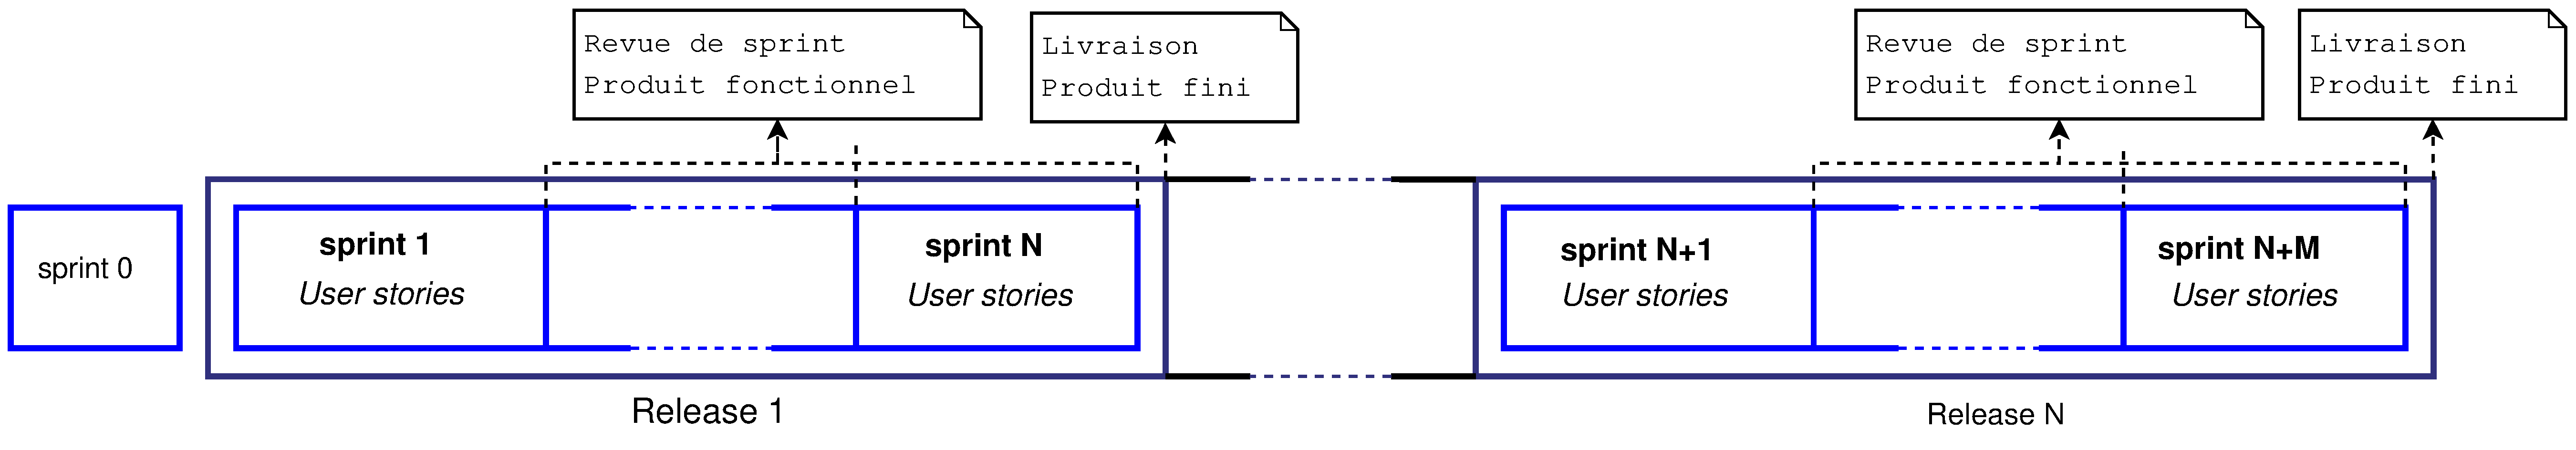
\includegraphics[width=18cm]{screens/scrum.eps}
	\caption{Fonctionnement des \key{Sprints} et \key{Releases} de la méthode \key{Scrum}}
\end{figure}

Outre les avantages qu'apporte la méthode \key{Scrum} à ce projet, l'équipe avait la volonté d’évoluer vers une méthode qui diffère de celles qui ont pu
être abordées en cours. Cette volonté est d’ailleurs confortée par le désir de découvrir  de nouvelles technologies (C++ et Qt jusque-là peu connus
par la majorité du groupe). 


\subsection{Application de la méthode \key{Scrum} et critères de qualité}
Dans le cadre de notre projet, la durée d'un \key{Sprint} a été défini à deux semaines. Un \key{Sprint}\index{Méthode Scrum!Sprint} est constitué de \key{User Stories}\index{Méthode Scrum!User story} et de 
\key{Technicals Stories}\index{Méthode Scrum!Technical Story} qui sont préalablement définies lors de réunions quotidiennes aussi appelées \key{mêlées}\index{Méthode Scrum!Mêlées}. Ces \key{mêlées} sont quotidiennes, nous
profitons de notre temps libre dans l’emploi du temps pour les organiser. Pour les jours où ce n’est pas possible, nous avons mis en place un salon
de discussion IRC.  

La définition des \key{Technical Stories} indique brièvement la fonction que l'on doit réaliser. Les \key{User Stories} sont quant à elles toujours posées
sous cette forme :

\begin{exemple}
	\textbf{En tant que} \texttt{[Personne(s) utilisant le logiciel]}\\
	\textbf{Je souhaite} \texttt{[La fonctionnalité que je désire avoir]}\\
	\textbf{Afin de} \texttt{[Objectif de la fonctionnalité]}
\end{exemple}

Chaque \key{Story} possède un poids, c'est-à-dire une valeur indiquant sa complexité et/ou le temps nécessaire afin de la mettre en œuvre. Le poids de
chacune des \key{Story} est déterminé durant les \key{mêlées}\index{Méthode Scrum!Mêlées} au moyen d’un « Planning poker ». Ceci permet à chacun d’exprimer la complexité d’une
\key{Story} à réaliser. Chacun justifie le choix du poids qu'il a affecté et après un éventuel débat, on affecte cette valeur à la \key{Story}. Celle-ci ne
peut être affectée qu'une fois que l'ensemble des membres de l'équipe se sont mis d’accord. Elle possède également une priorité précisant
l'importance d’intégrer cette \key{Story} ans le \key{Sprint}\index{Méthode Scrum!Sprint}. Cette priorité se fait au moyen de quatre niveaux d’importance : 

\begin{itemize}
	\item \textit{Must} : La \key{Story} doit obligatoirement être réalisée lors du \key{Sprint}
	\item \textit{Should} : La \key{Story} devra être réalisée (dans la mesure du possible)
	\item \textit{Could} : La \key{Story} pourra être réalisée car elle n’a aucun impact sur les autres tâches
	\item \textit{Would} : La \key{Story} ne sera pas nécessairement faite et sera alors reportée au prochain \key{Sprint}
\end{itemize}

Une  \key{Story} est considérée comme finie lorsqu'elle est fonctionnelle d’un point de vue utilisateur c'est-à-dire :
\begin{itemize}
	\item Les tests unitaires (pour la base de données ou pour les modèles) sont validés
	\item Les tests d’intégrations sont validés
	\item Lorsque chaque méthode est documentée
\end{itemize}

À la fin du \key{Sprint}, on présente à notre client, Monsieur Frédéric \bsc{Migeon}, afin qu'il le valide. Un \key{Sprint} fournit toujours :
\begin{itemize}
	\item une démonstration des nouvelles fonctionnalités logicielles
	\item des tests unitaires
	\item une documentation du code (au format HTML et PDF)
	\item un manuel d’utilisateur à jour des nouvelles fonctionnalités
\end{itemize}

Notre projet sera réalisé en deux \key{Releases}\index{Méthode Scrum!Release}, c'est-à-dire qu'il y aura deux versions livrables. Chacune de ces versions est composée de trois 
\key{Sprints}\index{Méthode Scrum!Sprint}  ayant chacun un poids moyen de 50 pour environ 10 \key{Stories}.

Les versions livrables du logiciel sont définies dans un carnet des produits (\key{Product Backlog}) qui référence l'ensemble des \key{Stories} des
différents \key{Sprints}. Ce carnet est susceptible d’évoluer en fonction des besoins du client, de nouveaux choix de conception ou encore d’éléments
n’ayant pas été prévu. 

\subsection{Organisation et rôles dans l'équipe de développement}
La méthode \key{Scrum} possède des rôles qui lui sont propres: le \key{Scrum Master}\index{Méthode Scrum!Scrum master}, le \key{Product Owner}\index{Méthode Scrum!Product Owner} et l'équipe de développement\index{Méthode Scrum!Équipe de développement}. 

\subsubsection{Scrum Master : Florent Berbie}
Le \key{Scrum Master}\index{Méthode Scrum!Scrum master} aura pour mission principale de guider les développeurs dans l'application de la méthode \key{Scrum}. Il veillera à ce que la méthode soit
comprise de tous et appliquée de façon correcte. Il aura le rôle de meneur lors de phases importantes d’application de la méthode telles que le
planning poker ou encore les mêlées quotidiennes.
\subsubsection{Product owner : Antoine de Roquemaurel}
Le \key{Product owner}\index{Méthode Scrum!Product owner} est la seule personne responsable du carnet de produit et de sa gestion. Ce dernier comprend l’expression de tous les items associés
à une priorité (l'importance pour le client). La compréhension de ceux-ci ainsi que la vérification du travail fourni est sous la responsabilité du
\key{Product owner}.
\subsubsection{Équipe de développement\index{Méthode Scrum!Équipe de développement} : Florent Berbie, Antoine de Roquemaurel, Cédric Rohaut, Andriamihary Razanajatovo}
Afin d’assurer une plus grande cohésion entre les membres de l’équipe, un même niveau d’implication et un travail de plus grande qualité nous avons
définis des rôles spécifiques : 
\subsubsection{Directeur qualité\index{Méthode Scrum!Directeur qualité} : Cédric Rohaut}
Le responsable qualité sera garant de la transposition des exigences du client sous forme de solutions techniques au sein du logiciel final. En
d’autres termes, il veillera à ce que le logiciel apporte une solution technique optimale pour le client. De plus il devra vérifier et valider la
qualité du logiciel au travers de tests, du respect des conventions et de l'aspect général du logiciel.

\subsubsection{Directeur documentation\index{Méthode Scrum!Directeur documentation} : Andriamihary Razanajatovo}
Le responsable documentation sera chargé de la révision de l'ensemble des documents avant leur remise ou leur soumission aux parties prenantes
concernées. Il veillera à la qualité des aspects fondamentaux, à savoir le fond et la forme, des documentations à fournir.

\subsubsection{Directeur technique\index{Méthode Scrum!Directeur technique} Qt, C++ : Antoine de Roquemaurel}
Le responsable technique Qt, C++ sert de support à l'équipe en cas de problèmes techniques liés au développement sur la plate-forme Qt. De par ses
connaissances acquises dans ce domaine, il sera le plus à même à aider les membres de l'équipe projet ayant des difficultés avec cette technologie.
De plus, dans le but de minimiser les couplages lors de la conception, il veillera à ce que le patron de conception MVC\footnote{Modele, Vue, Contrôleur} soit correctement utilisé. Ainsi, le code
sera clairement découpé en trois parties : modèle, vue et contrôleur ce qui permettra de s’assurer des contrôles d'interactions entre nos composants
logiciels.

\subsubsection{Autres rôles et responsabilités de chaque développeur et organisation/fonctionnement général}
Dans un souci d’assurance qualité, chaque responsable est en mesure de présenter les difficultés qu'il a eu à gérer, de présenter les différents
solutions possibles à ce problème et de justifier le choix de la technique adoptée.

Lors de la réalisation d’un cas d’utilisation (\key{issue}\index{Méthode Scrum!Issue} sur \key{Github}), celui-ci est assigné à un développeur. Une fois que ce dernier considère sa
tâche comme finie, il indique (via une \key{Pull Request}) aux autres membres de l’équipe que la tâche est soumise à la validation et à l'intégration.
Un des autres membres vérifie que la fonction est conforme à sa description, que le code est facilement compréhensible et correctement commenté. Dans
le cas ou la revue de code ne donne pleine satisfaction, le membre effectuant cette revue et les autres membres de l’équipe pourront ajouter des
commentaires pour débattre de la fonctionnalité, de l’implémentation de la fonction ou des technologies employées pour y résoudre. Chacun pourra
alors soumettre sa vision du problème et la manière avec laquelle il aurait résolu le problème. 

\section{Les Technologies utilisées}
\subsection{Architecture Logicielle}
L’objectif du logiciel est d’éditer des devis\index{FactDev!Devis} et factures\index{FactDev!Facture} et de proposer une gestion de ses clients\index{FactDev!Gestion des clients} : le client possède un ou plusieurs projets auxquels sont associés un ou plusieurs devis et/ou factures. 
De ce fait, l’architecture logicielle comporte une base de données de type SQLite\index{Outils!SQLite} pour la gestion des clients, de ses projets, des devis et factures associés à chacun des projets et des prestations propres à chaque devis et facture. 
Nous utilisons un patron de conception MVC, avec un modèle qui correspond aux objets métiers Client, Projet, Factures, Devis, Prestations. Ces objets sont instanciés par les classes associées à la base de données qui réalisent ces tâches.
Enfin nous générerons les devis et factures en LaTeX ou en PDF.

\subsection{Environnement de développement}
Le logiciel est développé à partir du \key{framework}
\footnote{Ensemble de composants logiciels structurels servant à créer les fondations d'une future application. Un framework est créé par des développeurs pour d'autres développeurs. Un framework peut être vu comme une boîte à outils.} 
Qt(version 5)\index{Outils!Qt}
en langage de programmation C++ (version 11) avec l'EDI\footnote{Environnement de Développement Logiciel} Qt Creator (version 3.3)\index{Outils!Qt Creator}. 

Les membres de l’équipe développent sur différents systèmes : MAC OS (OS X 10.10), Linux (Fedora 20 et Linux Mint 17.1). Bien que développé uniquement sur des systèmes UNIX, l’application sera compatible avec Windows. 

Afin de mener au mieux ce projet, l’équipe utilise l’outil \key{Github}, un service web d’hébergement et de gestion de développement de logiciels. 

\subsection{Outils pour la Gestion de Projet Agile}
La développement de notre logiciel s’appuie sur \key{Github}\index{Outils!Github} qui permet la gestion des différentes versions de notre logiciel. 
Cet outil est composé d’une branche directrice (appelée \key{Master}), sur laquelle se greffe de nouvelles branches : une branche par \key{Sprint}\index{Méthode Scrum!Sprint}. L’ensemble des \key{User Stories}\index{Méthode Scrum!User Story} que nous avons défini sont représentées dans \key{Github} par des \key{Issues}. Chaque \key{Issue} fait l’objet d’une nouvelle branche provenant de celle du Sprint associé. L’avantage que propose cette gestion permet à chacun de développer de son côté sans entrer en conflit avec les autres membres de l’équipe. Une fois l’issue terminée et validée par la revue de code, l’on fusionne la branche de l’issue à celle du Sprint associée afin que l’équipe bénéficie de la nouvelle version, stable et fonctionnelle. On procède de la même façon en fin de \key{Sprint} en intégrant la branche de \key{Sprint} à la branche principale \key{Master}.

\begin{figure}[H]
	\centering
	\includegraphics*[width=12cm]{screens/BranchingWorkflow.eps}
	\caption{Principe du « Git Branching Workflow »}
\end{figure}

Outre la gestion des différentes versions de notre code, \key{Github} permet un suivi de notre projet. Le site internet \key{Github} dédié au projet est accessible à l’équipe et notre client Monsieur Frédéric \bsc{Migeon}. 
De plus, \key{Github} contient un Wiki avec les règles de bonne conduite et les conventions à respecter pour assurer l’homogénéité de notre projet. 

\subsection{Documentation\index{Documentation}}
La centralisation des documents se fait au moyen du Wiki\index{Documentation!Wiki} de \key{Github} et de Google Drive. 
Le Wiki de \key{Github} contient :
Tutoriel sur les méthodes de travail (Git, Scrum, C++)
Convention de code à respecter (conventions de nommage des variables, des méthodes, d’organisation du code...)
Tutoriel sur la documentation (\key{Doxygen})\index{Documentation!Doxygen}.

Sur Google Drive, on trouve l’ensemble des documents à rédiger en équipe. Cet outils permet notamment d’éditer un même document à plusieurs et d’être facilement accessible par tout le monde. Parmi les documents accessibles sur le Drive, on trouve :
\begin{itemize}
	\item le manuel de l’utilisateur\index{Documentation!Manuel de l'utilisateur}
	\item le plan d'assurance qualité\index{Documentation!Plan d'assurance qualité}
	\item le Carnet des produits \key{Product Backlog}\index{Documentation!Product Backlog}
	\item les graphiques d’avancement:\index{Graphqiues d'avancement}
	\begin{itemize}
		\item Burndown chart\index{Documentation!Graphqiues d'avancement!Burndown chart}
		\item Burnup chart\index{Documentation!Graphqiues d'avancement!Burnup chart}
	\end{itemize}
	\item les Comptes rendus mensuels\index{Documentation!Comptes rendus mensuel}
	\item d’autres documents concernant le projet mais n’étant parmi ceux à rendre
\end{itemize}
 
\subsection{Assurance de la qualité du code}
Pour assurer une meilleure homogénéité, lisibilité et maintenabilité du code, nous utilisons l’outil \key{SonarQube}\index{Outils!SonarQube}, un logiciel permettant de mesurer la qualité du code source  en continu. 
//Celui-ci analyse et fournit diverses informations sur le code tel que:
\begin{itemize}
	\item le pourcentage de code non documenté (ou pas assez documenté)
	\item la complexité générale du logiciel ou, au car pas car, des méthodes de notre programme
	\item le bon respect des conventions de codages (nommage des attributs/méthodes, indentation, …)
	\item la couverture de code (via les tests unitaires) la duplication de code
\end{itemize}
	\appendix
	\listoffigures
	\printindex

\end{document}
